\begin{figure*}
  \centering
    \begin{subfigure}[b]{0.3\textwidth}
        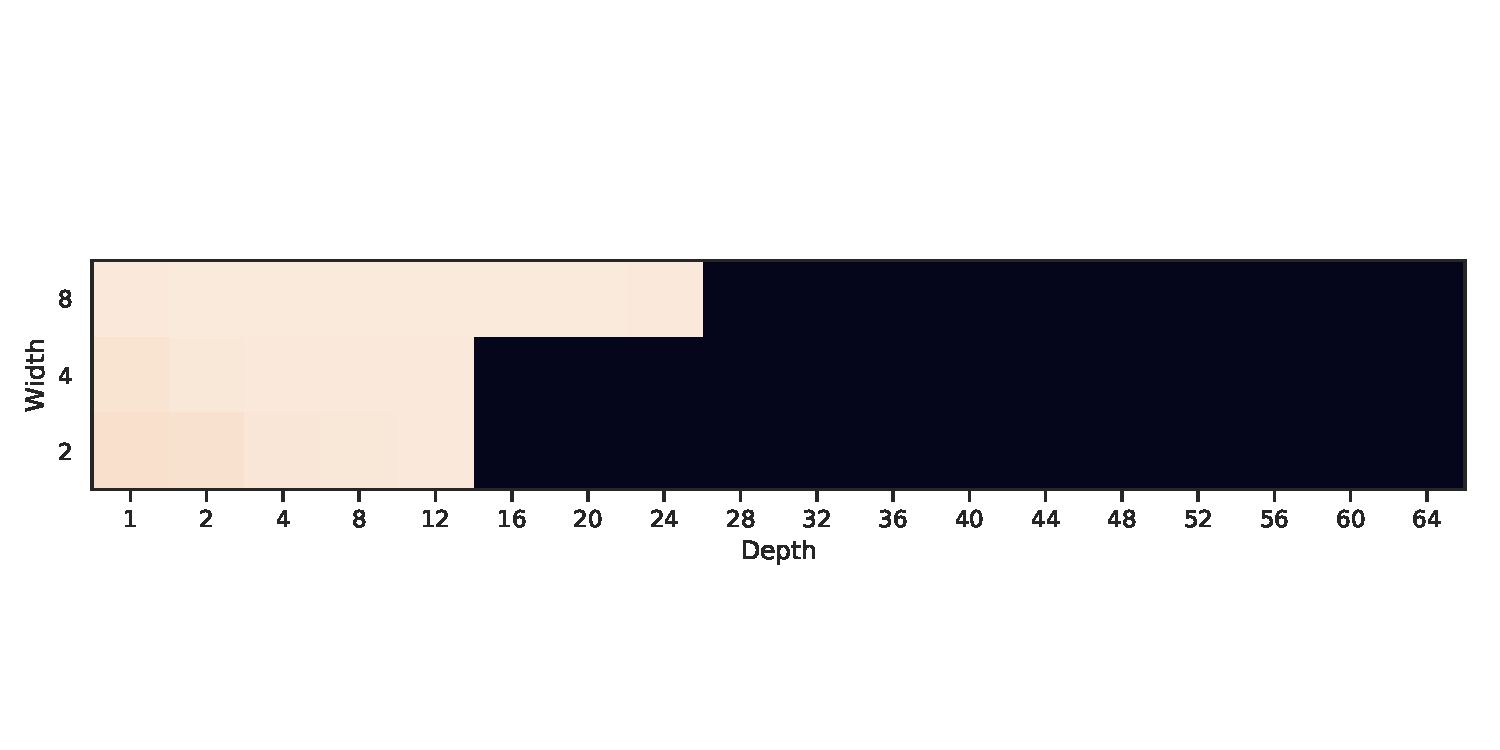
\includegraphics[width=\textwidth]{img/mnist_grid/acc-relu-ks-3x3-bs-1024.pdf}
        \caption{\ReLU}
        \label{fig:mnist_grid_relu}
    \end{subfigure}
    ~ %add desired spacing between images, e. g. ~, \quad, \qquad, \hfill etc. 
      %(or a blank line to force the subfigure onto a new line)
    \centering
    \begin{subfigure}[b]{0.3\textwidth}
        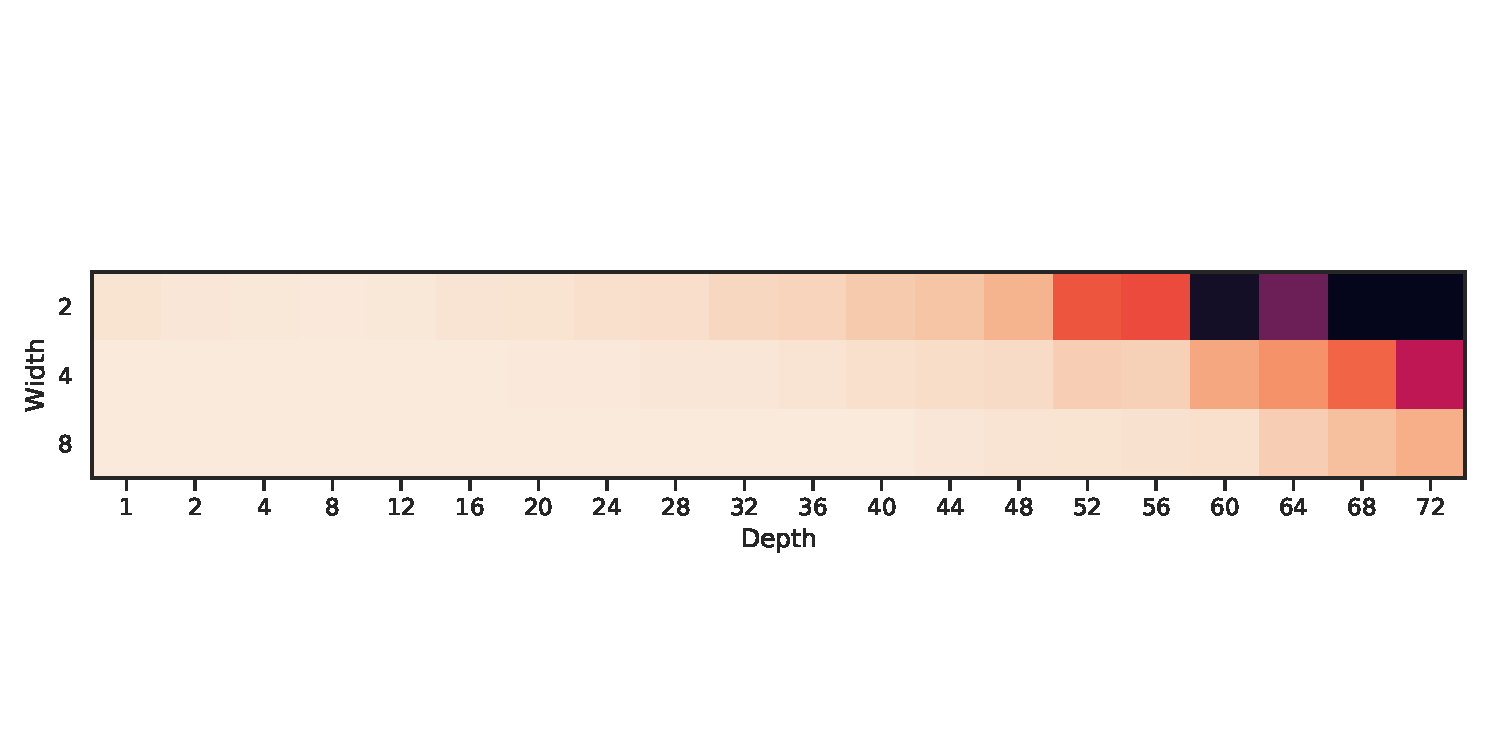
\includegraphics[width=\textwidth]{img/mnist_grid/acc-relu-bn-ks-3x3-bs-1024.pdf}
        \caption{\ReLUBN}
        \label{fig:mnist_grid_relubn}
    \end{subfigure}
    ~ %add desired spacing between images, e. g. ~, \quad, \qquad, \hfill etc. 
      %(or a blank line to force the subfigure onto a new line)
    \centering
    \begin{subfigure}[b]{0.3\textwidth}
        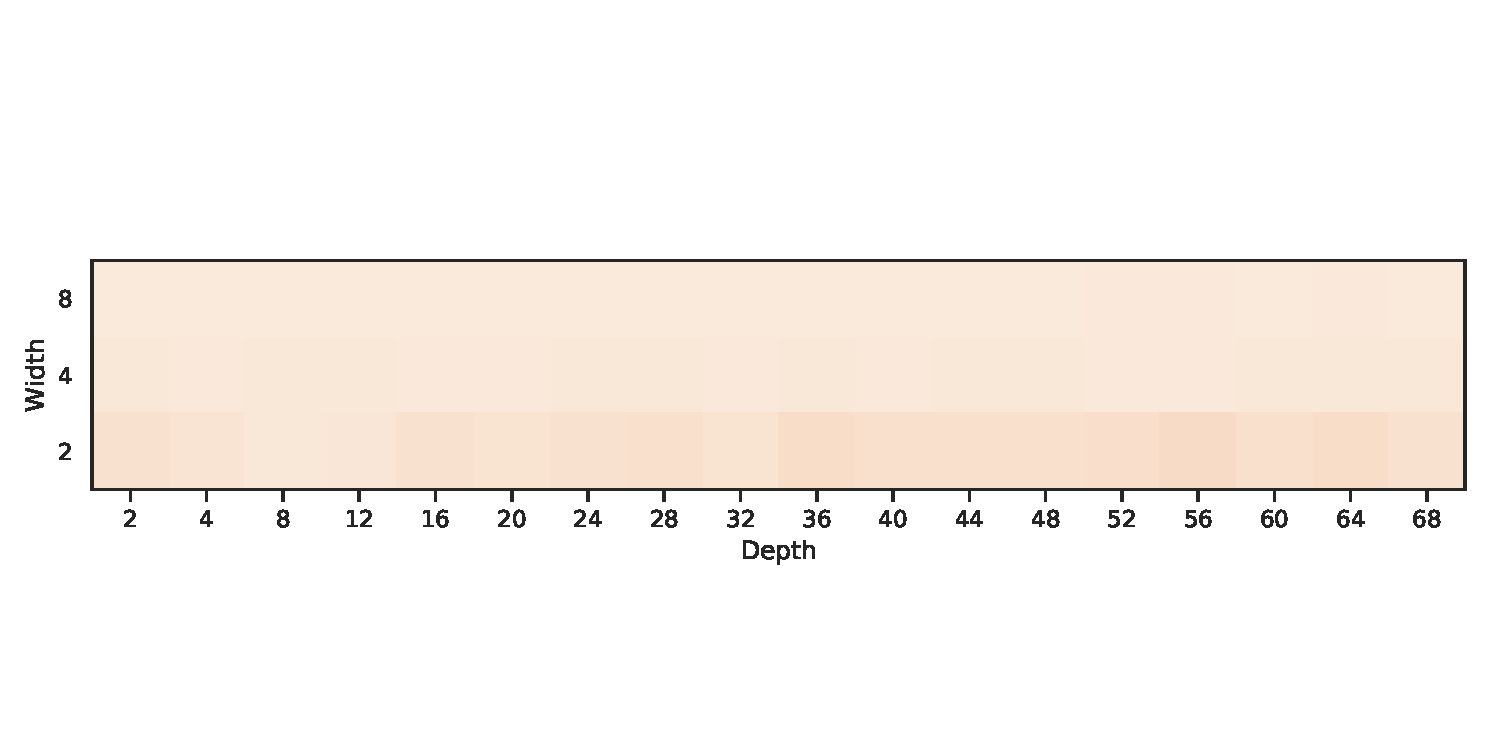
\includegraphics[width=\textwidth]{img/mnist_grid/acc-sep-up-1e-08-ks-3x3-bs-1024.pdf}
        \caption{\SepUnitPoint}
        \label{fig:mnist_grid_up}
    \end{subfigure}
    ~ %add desired spacing between images, e. g. ~, \quad, \qquad, \hfill etc. 
      %(or a blank line to force the subfigure onto a new line)
    
  \caption{Depth vs Width accuracy plot a for rectangular network using a grid (width from $2$ to $25$ and depth from $2$ to $150$),  trained using a Adam learning rate of $0.01$ in the MNIST dataset. The color show the accuracy attained of each of the combinations of width and depth, the clearer the better. Notice how \ReLU, Figure \ref{fig:mnist_grid_relu}, fails with networks deeper than 30 layers. In other hand, \ReLUBN, Figure \ref{fig:mnist_grid_relubn}, manages to work until 70 layers deep. \SepUnitPoint,  Figure \ref{fig:mnist_grid_up}, works significantly better than both, up to 120 layers. Notice how all the methods suffer from degradation from depth, which is partially alleviated by the use of greater width. This is consistent with \cite{simpnet} and \cite{densenet}. However, \SepUnitPoint is able to delay the apparition of the issue. This is especially visible when the number of units is small (from $2$ to $5$) where \ReLUBN fails to work whereas \SepUnitPoint does not.}
  \label{fig:mnist_grid} 
\end{figure*}
